\documentclass{article}
\textheight 23.5cm \textwidth 15.8cm
%\leftskip -1cm
\topmargin -1.5cm \oddsidemargin 0.3cm \evensidemargin -0.3cm
%\documentclass[final]{siamltex}

\usepackage{verbatim}
\usepackage{fancyhdr}
\usepackage{graphicx}
\usepackage{framed} 
%\pagestyle{fancy} \lhead{FDM Homework Template} \chead{}
%\rhead{\bfseries Yan XU}
%
%\lfoot{} \cfoot{} \rfoot{\thepage}
%\renewcommand{\headrulewidth}{0.4pt}
%\renewcommand{\footrulewidth}{0.4pt}
%

%利用TEX排版系统的CTEX中文套装
\usepackage[UTF8,noindent]{ctex}
%等式对齐
\usepackage{amsmath}
\usepackage{amssymb}

\title{OpenGL入门}
\author{陈柯}

\begin{document}
	\maketitle
	
	\section{目的}
	利用UGL框架实现:
	
	1. 实现 normal map 和 displacement map;
	
	2. 利用 displacement map 在 vertex shader 中进行简单降噪;
	
	3. 实现阴影映射
	\section{方法}
	\subsection{法向贴图}
	典型使用方式如下:
	\begin{figure}[htb]
		\caption{\label{table.label} 法向贴图原理} \centering
		\begin{center}
			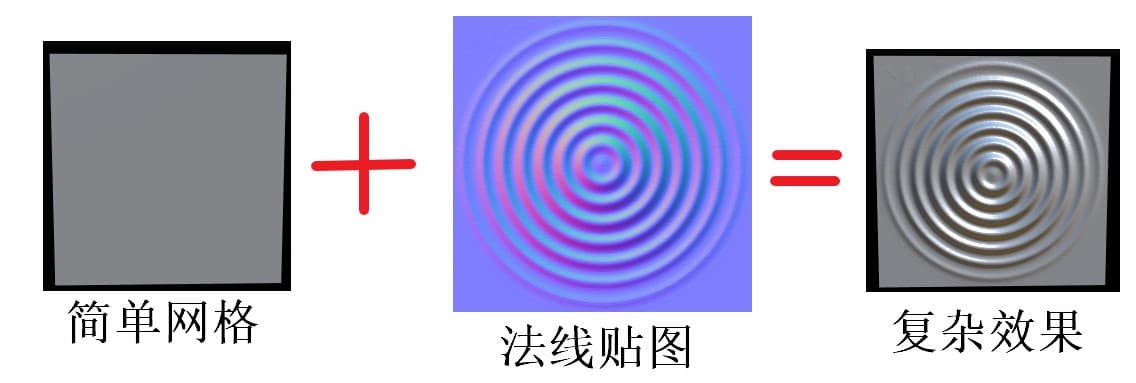
\includegraphics[width=6in]{normal_map_usage.jpg}
			\label{figure.label}
		\end{center}
	\end{figure}
	
	其中法线贴图在渲染中用于改变原法向,从而影响着色效果。法线贴图一般为蓝紫色,这是因
	为贴图中的法向是定义在切空间中的,上方向为 z 方向,对应于 RGB 的 B 通道。
	\subsection{置换贴图}
	典型使用方式如下:\clearpage
	\begin{figure}[htb]
		\caption{\label{table.label} 置换贴图原理} \centering
		\begin{center}
			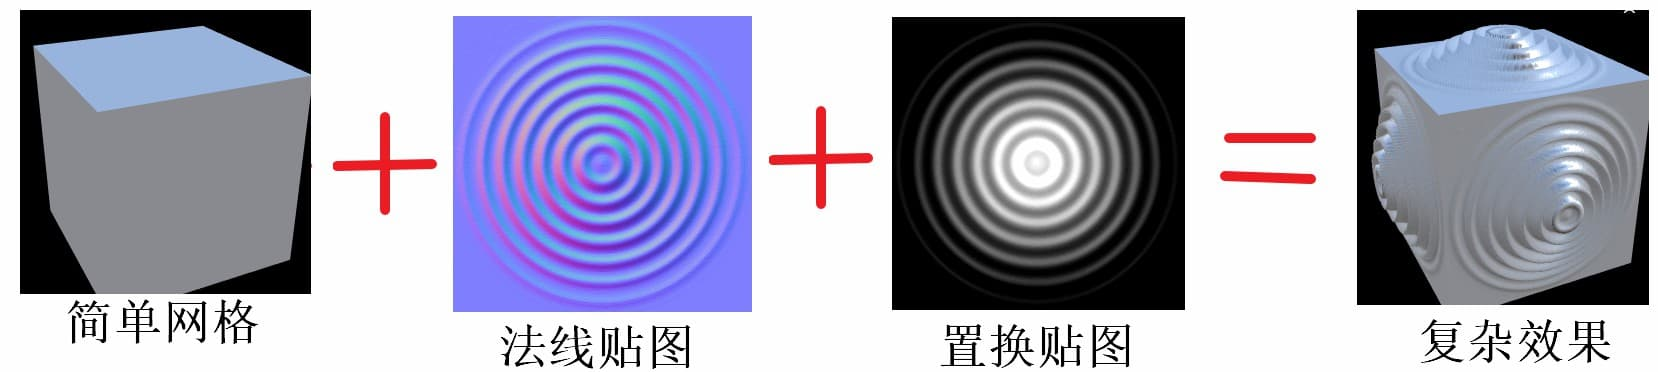
\includegraphics[width=6in]{displacement_map_usage.jpg}
			\label{figure.label}
		\end{center}
	\end{figure}

	其中置换贴图用于改变顶点的位置,0 (黑色)表示不动,1(白色)表示沿着法向偏移。
	
	将置换贴图的值转换成顶点偏移量的方式是自定义的,示例如下:
	
	- 0-0.5 为下沉,0.5-1.0 为凸起,变化量用一个系数决定
	
	- 0-1.0 为凸起,变化量用一个系数决定
	
	- 上边两种方式可范化成:displacement = lambda * (bias + scale * pixel value)
	
	- displacement = lambda * (-1 + 2 * pixel value)
	
	- displacement = lambda * (0 + 1 * pixel value)
	
	由于要改变顶点坐标,在实时渲染中应在 vertex shader 中采样置换贴图来偏移顶点,因此
	简单网格应含有大量的内部顶点。
	
	由于置换贴图只改变了顶点的位置,不改变顶点的法向,所以,如果不添加相应的法线贴图的
	话,渲染效果不太正确,如下:
	\begin{figure}[htb]
		\caption{\label{table.label} 置换贴图不改变法线的情况} \centering
		\begin{center}
			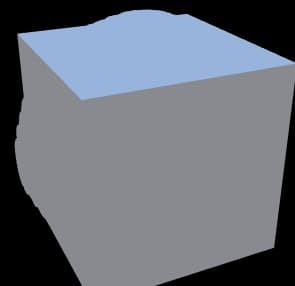
\includegraphics[width=4in]{displacement_map_error.jpg}
			\label{figure.label}
		\end{center}
	\end{figure}

	\subsection{用置换贴图进行简单去噪}
	项目提供的模型和加了随机噪声之后的模型如下
	\begin{figure}[htbp]
		\centering
		\begin{minipage}{0.49\linewidth}
			\centering
			\caption{原模型}
			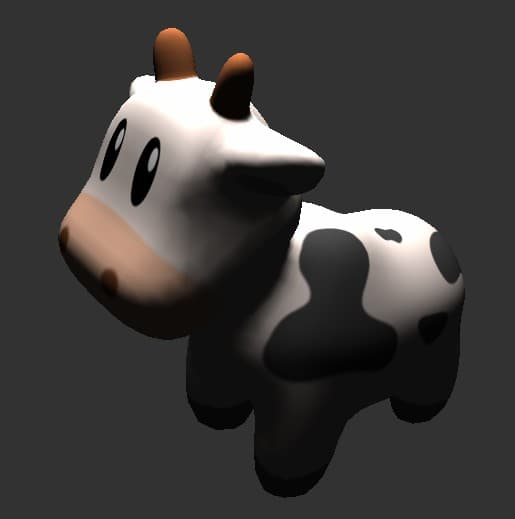
\includegraphics[width=1\linewidth]{spot.jpg}
			\label{chutian1}%文中引用该图片代号
		\end{minipage}
		%\qquad
		\begin{minipage}{0.49\linewidth}
			\centering
			\caption{加了噪声的模型}
			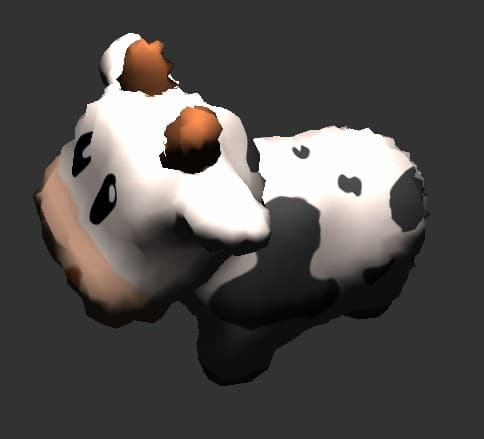
\includegraphics[width=1\linewidth]{spot_noise.jpg}
			\label{chutian2}%文中引用该图片代号
		\end{minipage}
	\end{figure}

	虽然给顶点加了噪声,但法线还是用了原本的,所以含噪声模型在渲染的不同主要体现在纹理
	的扭曲和边缘的凹凸不平上。我们只需将顶点进行合理的偏移就能达到不错的去噪效果。步骤
	如下:

	1. 计算每个顶点的偏移量:
	$$\delta_i=p_i-\frac{1}{|N(i)|}\sum_{j\in N(i)}p_j$$
	
	2. 将偏移量投影到法向上:
	$$\bar{\delta}_i=\langle\delta_i,\pmb{n}_i\rangle \pmb{n}_i$$

	3. 对每一个顶点进行偏移:
	$$\bar{p}_i=p_i-\lambda 
	\bar{\delta}_i=p_i-\lambda\langle\delta_i,\pmb{n}_i\rangle \pmb{n}_i$$
	
	4. 我们将 $\langle\delta_i,\pmb{n}_i\rangle$ 存到置换贴图中,注意设置好 bias 
	和 scale 将值变换到 0 和 1 之间

	简单来说,每个顶点有纹理坐标,将图像中该位置设为 bias 和 scale 后的 
	$\langle\delta_i,\pmb{n}_i\rangle$。
	
	我们需要注意的是,图像是离散的,只按上述做法难免出现重合、缺漏等,因此要根据每个顶
	点的偏移量,合理插值出整个置换贴图(比如 K 近邻加权均值,最近邻等)。
	\subsection{阴影映射}
	阴影映射(Shadow Mapping)背后的思路非常简单:我们以光的位置为视角进行渲染,我们能看
	到的东西都将被点亮,看不见的一定是在阴影之中了。假设有一个地板,在光源和它之间有一
	个大盒子。由于光源处向光线方向看去,可以看到这个盒子,但看不到地板的一部分,这部分
	就应该在阴影中了。
	\begin{figure}[htb]
		\caption{\label{table.label} 阴影映射原理} \centering
		\begin{center}
			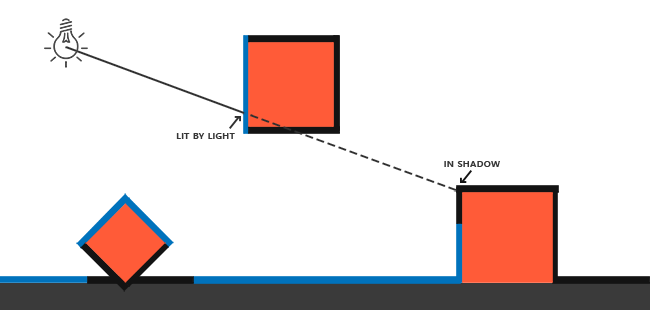
\includegraphics[width=4in]{shadow_mapping_theory.png}
			\label{figure.label}
		\end{center}
	\end{figure}
	这里的所有蓝线代表光源可以看到的fragment。黑线代表被遮挡的fragment:它们应该渲染为
	带阴影的。如果我们绘制一条从光源出发,到达最右边盒子上的一个片段上的线段或射线,那
	么射线将先击中悬浮的盒子,随后才会到达最右侧的盒子。结果就是悬浮的盒子被照亮,而最
	右侧的盒子将处于阴影之中。
	
	我们希望得到射线第一次击中的那个物体,然后用这个最近点和射线上其他点进行对比。然后
	我们将测试一下看看射线上的其他点是否比最近点更远,如果是的话,这个点就在阴影中。

	\section{实现结果}
	\subsection{法向贴图}
	
	\begin{figure}[htb]
		\caption{\label{table.label} CG字样的法向贴图} \centering
		\begin{center}
			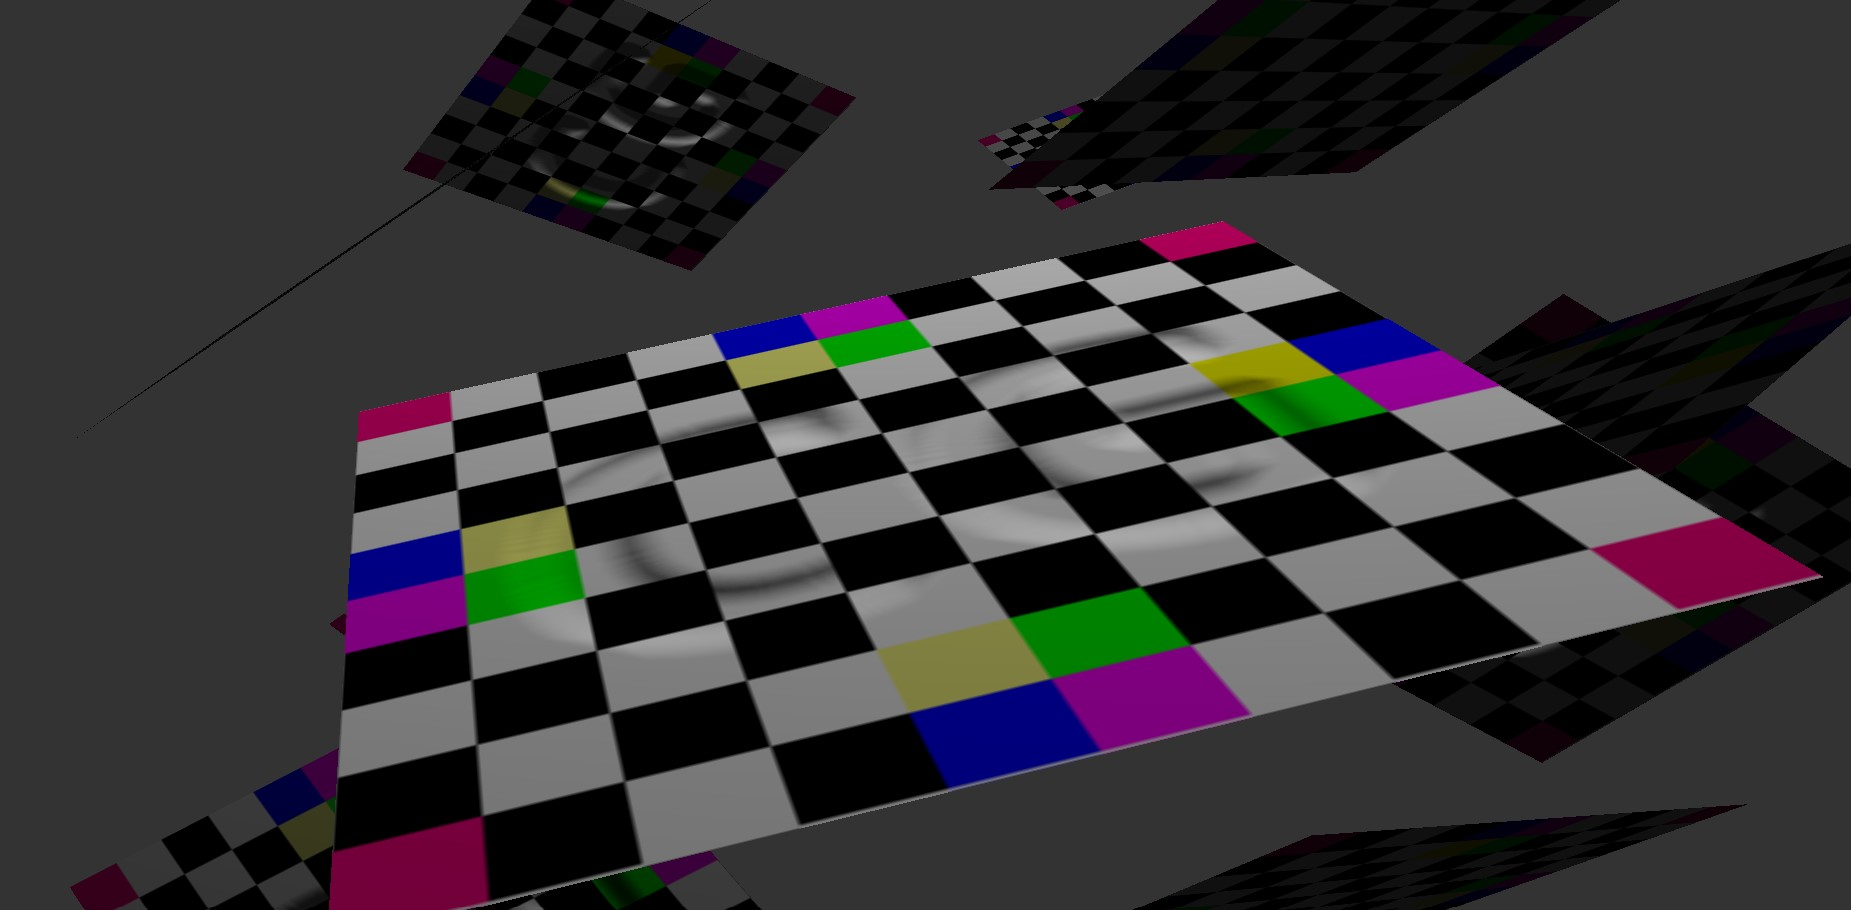
\includegraphics[width=5in]{normal1.jpg}
			\label{figure.label}
		\end{center}
	\end{figure}
	\begin{figure}[htb]
		\caption{\label{table.label} 人物图片的法向贴图} \centering
		\begin{center}
			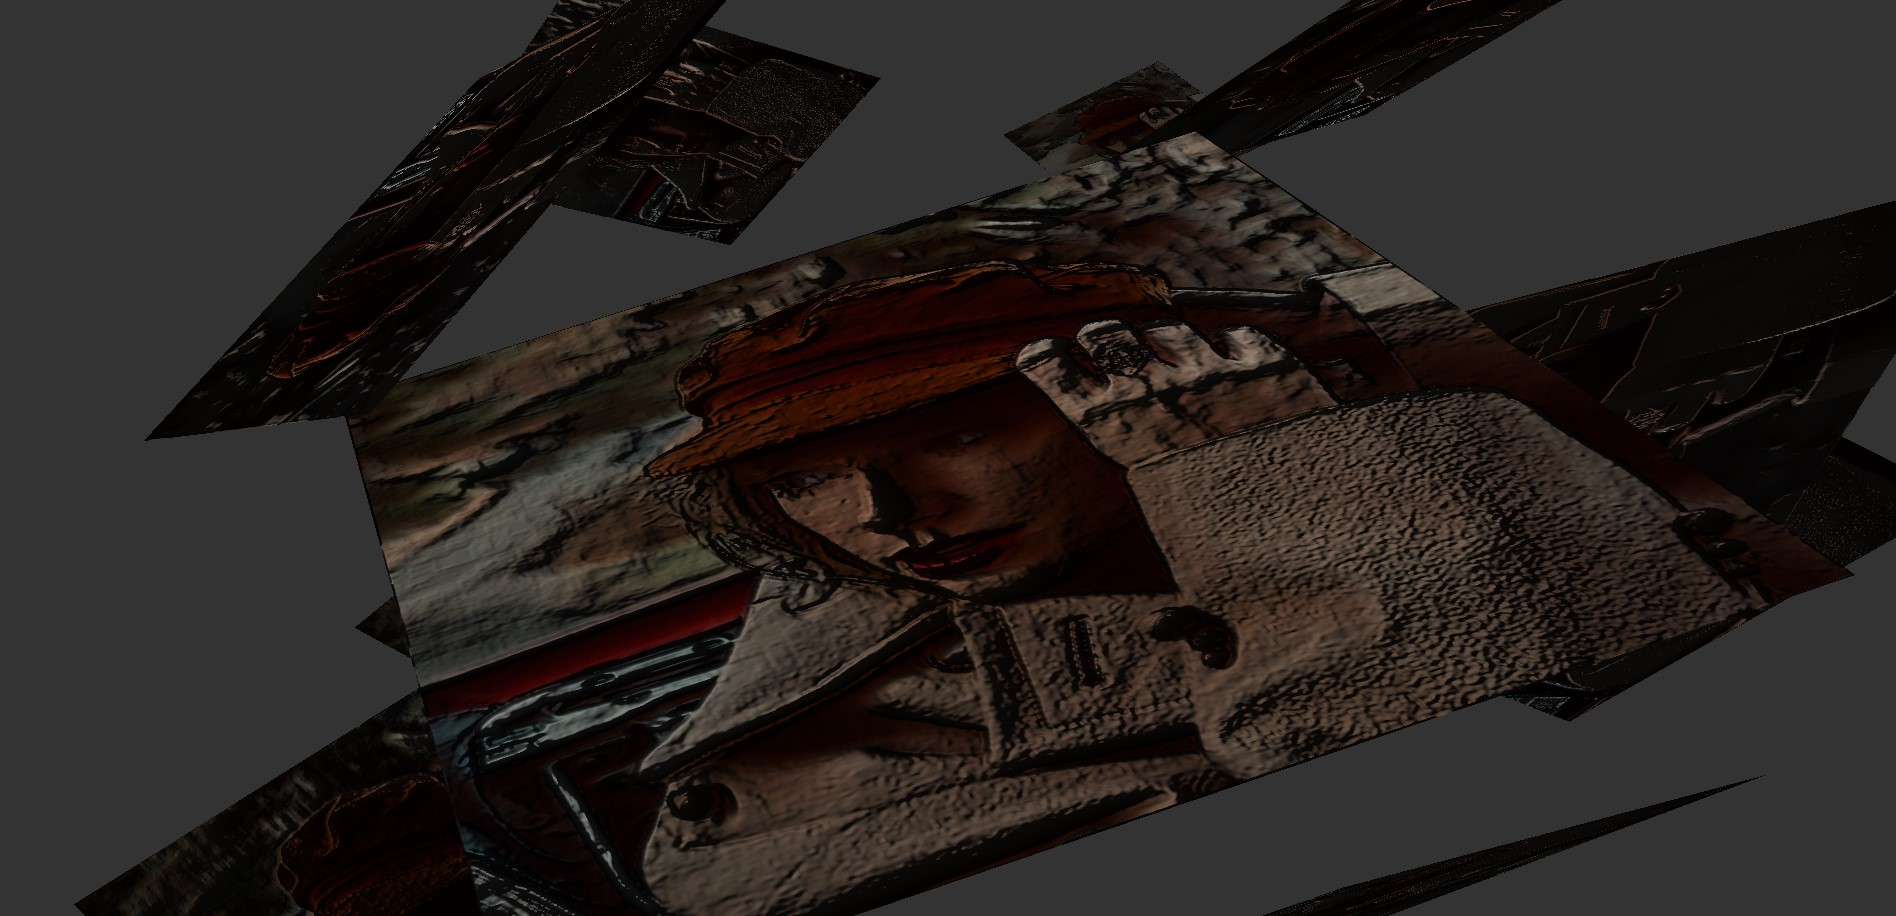
\includegraphics[width=5in]{normal2.jpg}
			\label{figure.label}
		\end{center}
	\end{figure}
	\begin{figure}[htb]
		\caption{\label{table.label} 文字的法向贴图} \centering
		\begin{center}
			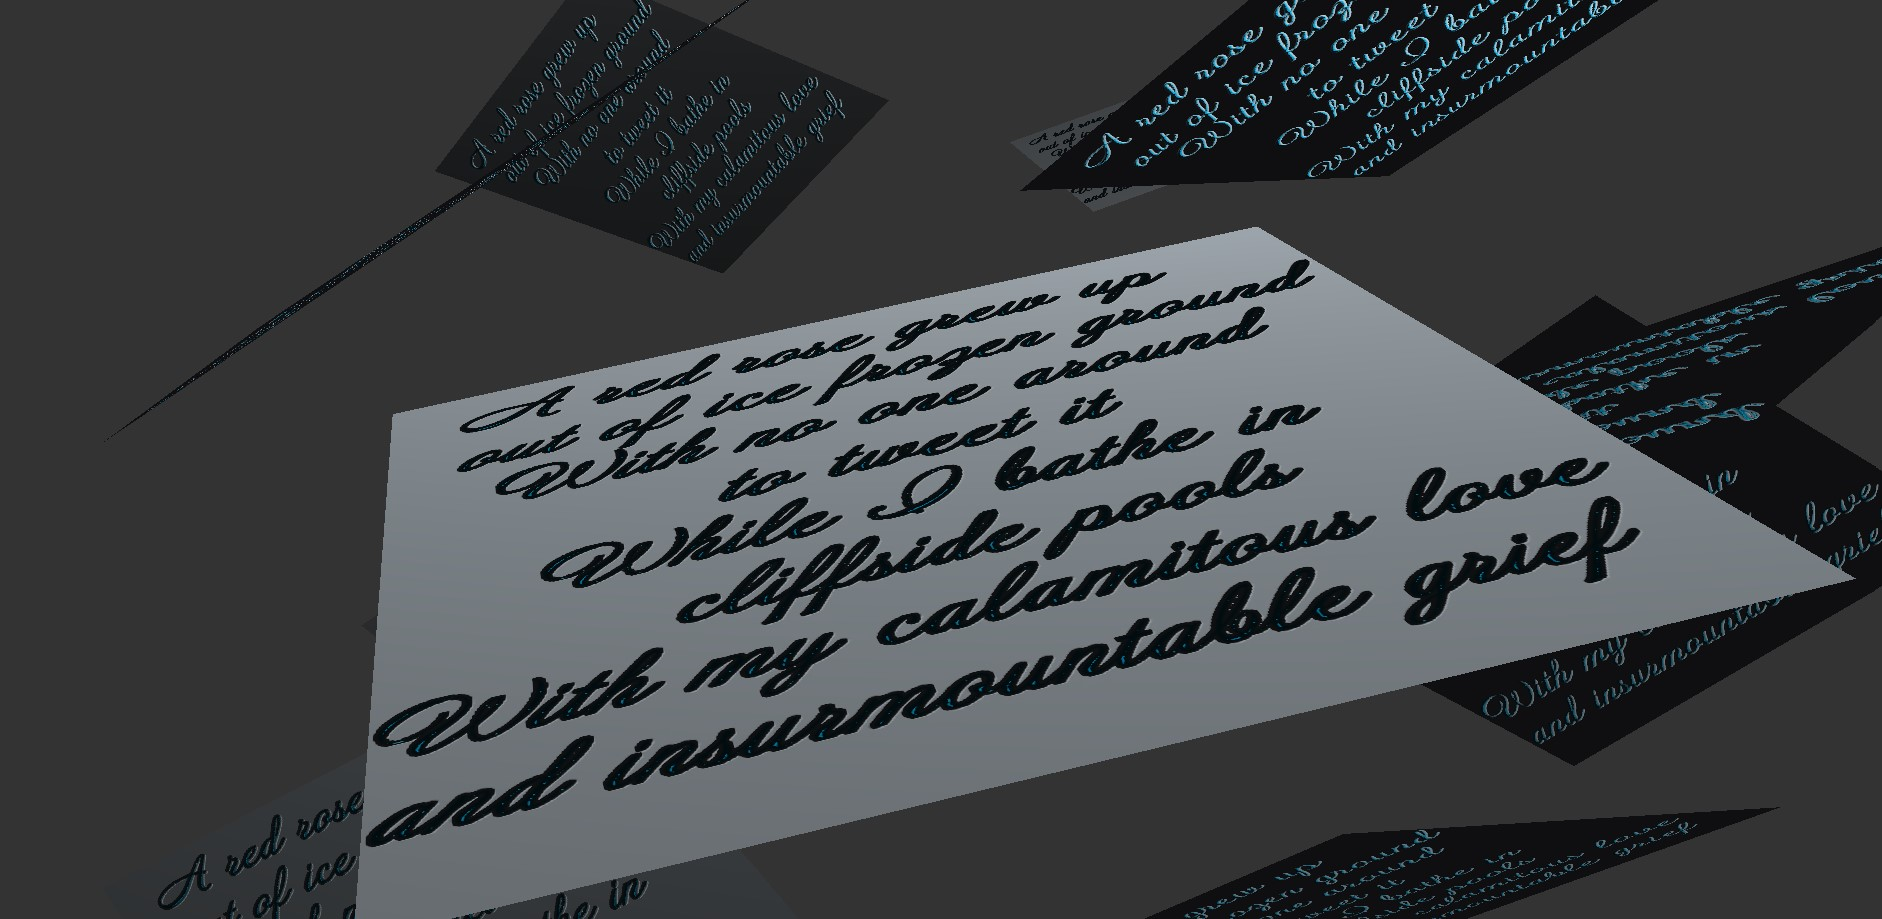
\includegraphics[width=5in]{normal3.jpg}
			\label{figure.label}
		\end{center}
	\end{figure}
	\clearpage
	\subsection{置换贴图}
	
	\begin{figure}[htb]
		\caption{\label{table.label} CG字样的置换贴图} \centering
		\begin{center}
			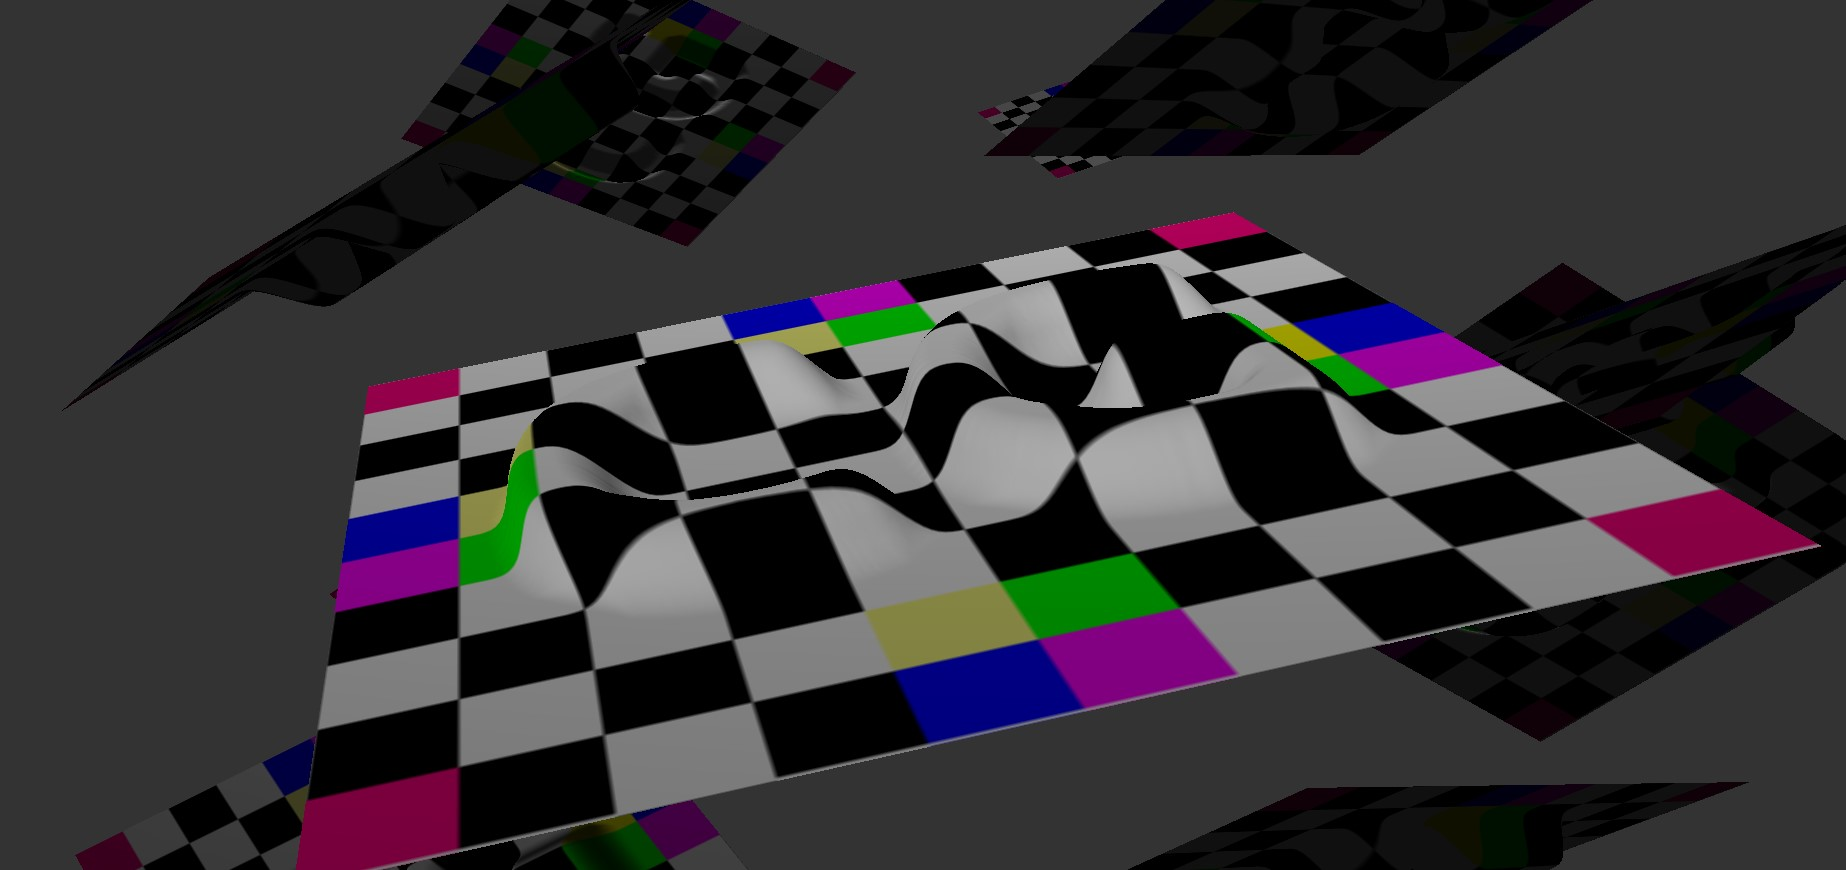
\includegraphics[width=5in]{displace.jpg}
			\label{figure.label}
		\end{center}
	\end{figure}
	
	
	
	\subsection{用置换贴图进行简单去噪}
	以下为原本的模型:
	\begin{figure}[htb]
		\caption{\label{table.label} 有噪声的模型} \centering
		\begin{center}
			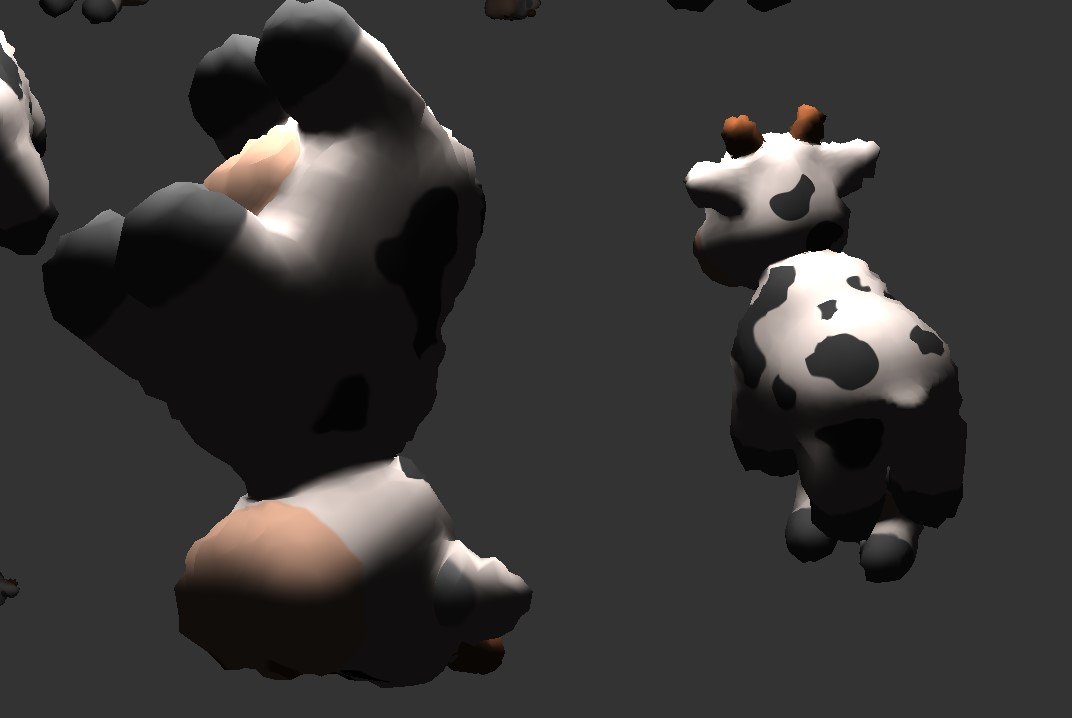
\includegraphics[width=5in]{noise.jpg}
			\label{figure.label}
		\end{center}
	\end{figure}

	我调用ANN库来做图像插值:下面是我根据算法实现的去噪后的模型:\clearpage
	\begin{figure}[htb]
		\caption{\label{table.label} 去噪后的模型} \centering
		\begin{center}
			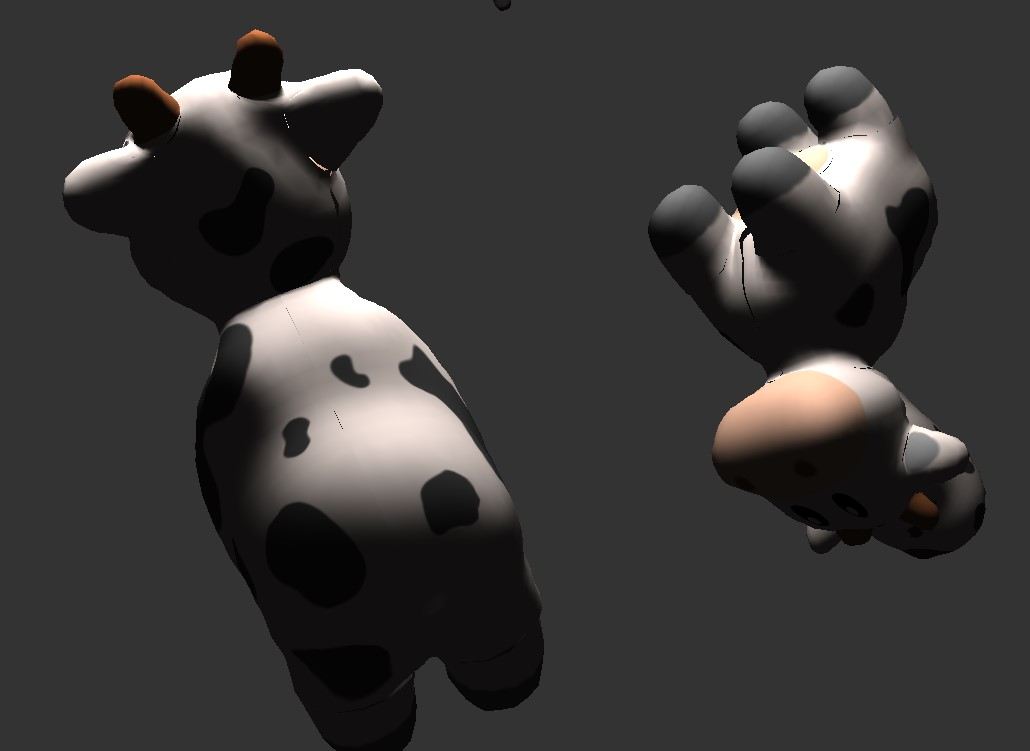
\includegraphics[width=4in]{denoise1.jpg}
			\label{figure.label}
		\end{center}
	\end{figure}

	 其中生成的displacementmap如下图:
	\begin{figure}[htb]
		\caption{\label{table.label} displacementmap} \centering
		\begin{center}
			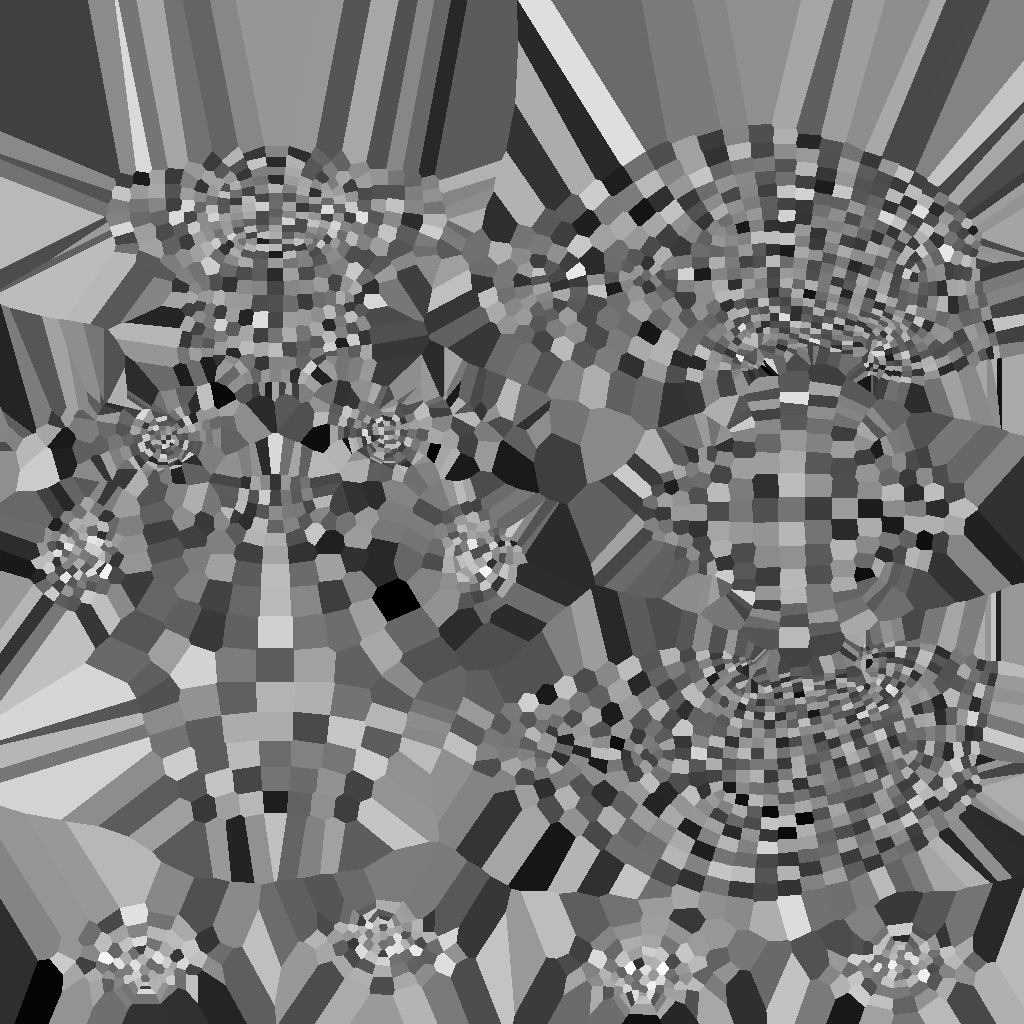
\includegraphics[width=2.8in]{1_denoise_displacement_map.png}
			\label{figure.label}
		\end{center}
	\end{figure}
	\clearpage
	根据我的调试发现此时displacement\_lambda=0.9f左右去噪效果最好。但是我们可以看到奶
	牛的背上,牛角处,肚子处等等都有裂缝。这里我们考虑可能是有许多顶点的世界坐标是相同
	的,法向也相同,纹理坐标不同。如下图:
	\begin{figure}[htb]
		\caption{\label{table.label} 有2个点世界坐标相同的情况} \centering
		\begin{center}
			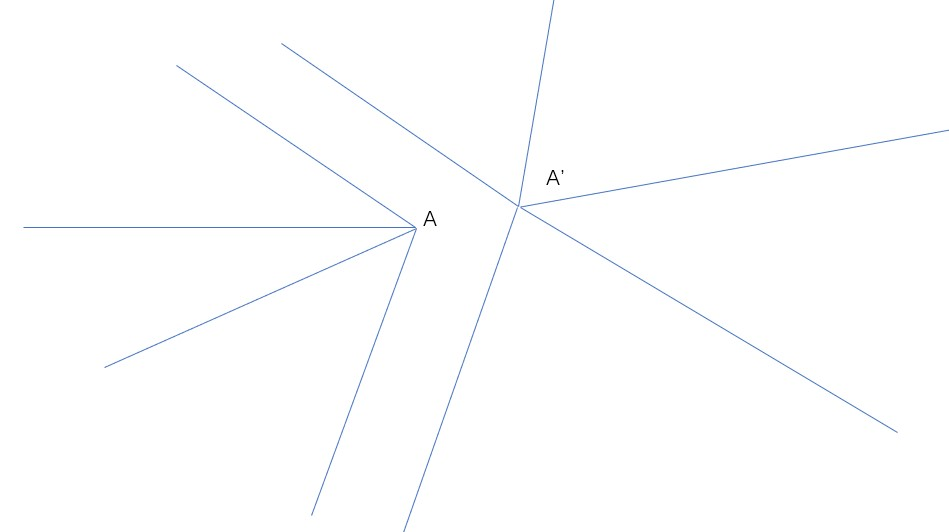
\includegraphics[width=3in]{overlap.jpg}
			\label{figure.label}
		\end{center}
	\end{figure}
	
	对于这种顶点,A和A’的邻结点应该是共有的。再把这种情况考虑进去我们可以得到:
	\begin{figure}[htb]
		\caption{\label{table.label} 去裂缝后的模型} \centering
		\begin{center}
			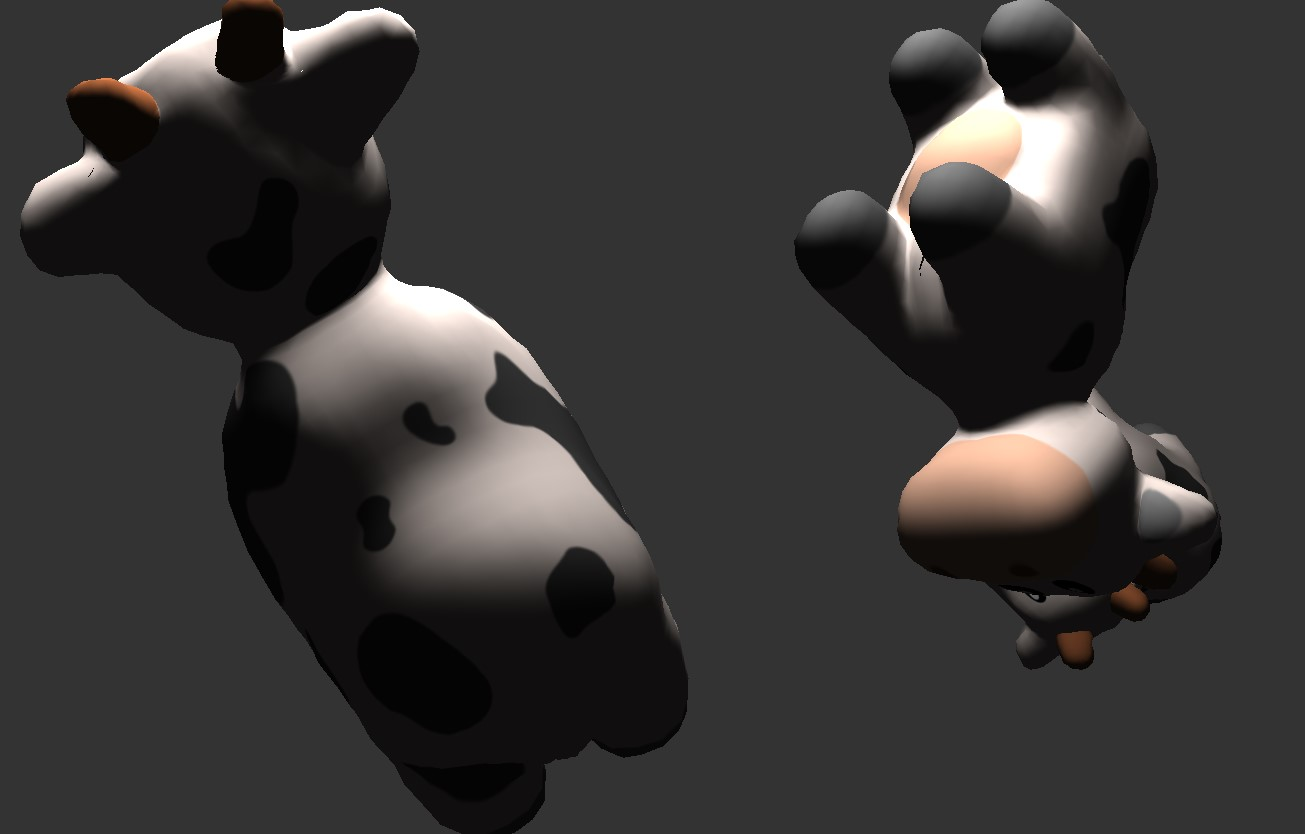
\includegraphics[width=5in]{denoise2.jpg}
			\label{figure.label}
		\end{center}
	\end{figure}

	我们可以看到奶牛背上的裂缝没有了,但是肚子上和牛角上还有少量裂缝,我们猜测可能是网
	格取纹理的时候本身就是不连续的,所以裂缝难以避免。
	\clearpage
	\subsection{阴影映射}
	利用助教的框架,再按照教程:
	
	https://learnopengl-cn.github.io/05\%20Advanced\%20Lighting/03\%20Shadows/01
	\%20Shadow\%20Mapping/
	
	我们可以实现阴影的渲染,由于阴影贴图助教已经实现好了,我们只需要在render loop里计
	算好矩阵lightProjection, lightView, 执行shadow\_program,再在片元着色器里渲染阴
	影就可以了。以下为实现的效果:
	\begin{figure}[htb]
		\caption{\label{table.label} 初步的阴影渲染} \centering
		\begin{center}
			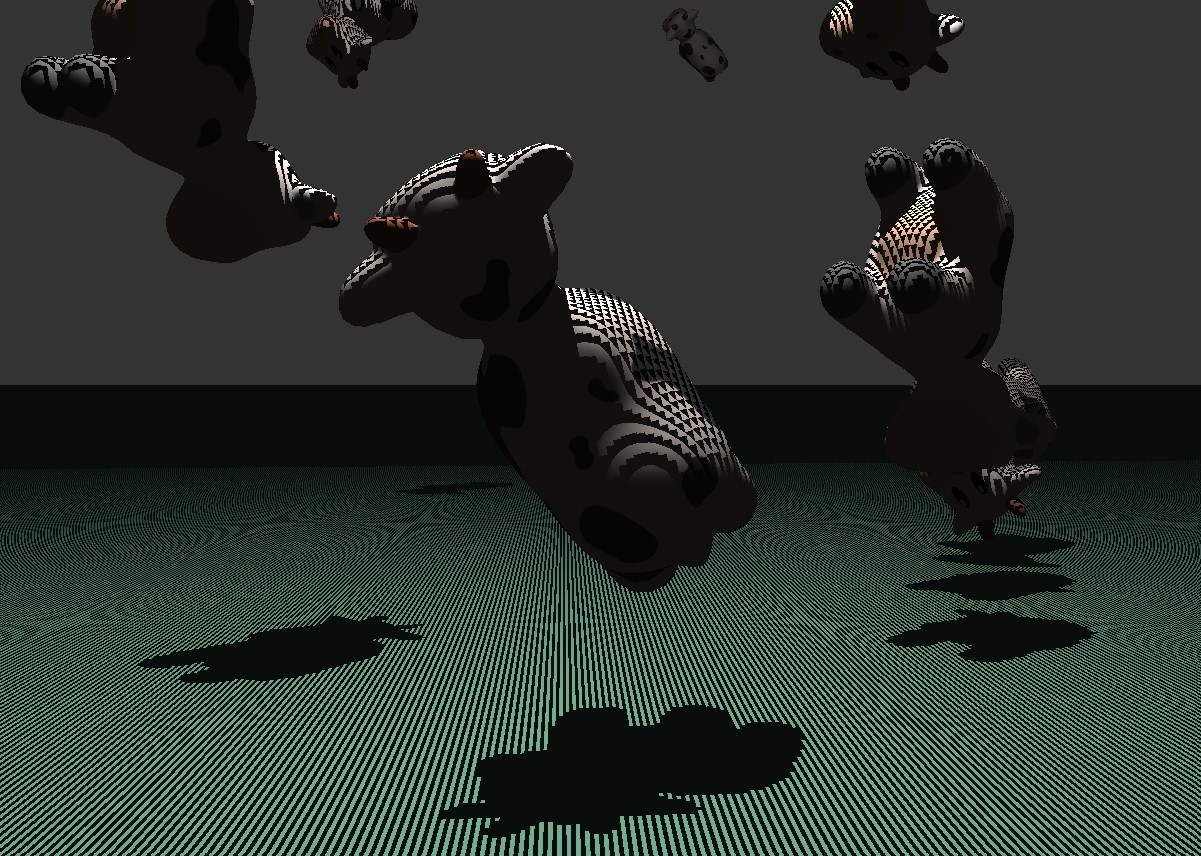
\includegraphics[width=4in]{shadow1.jpg}
			\label{figure.label}
		\end{center}
	\end{figure}
	
	我们可以看到地板四边形渲染出很大一块交替黑线。这种阴影贴图的不真实感叫做阴影失真
	(Shadow 
	Acne)。教程里也提供如何优化算法来消除失真。我们可以用一个叫做阴影偏移(shadow 
	bias)的技巧来解决这个问题,我们简单的对表面的深度(或深度贴图)应用一个偏移量,这
	样片段就不会被错误地认为在表面之下了。使用了偏移量后,所有采样点都获得了比表面深度
	更小的深度值,这样整个表面就正确地被照亮,没有任何阴影。我们可以这样实现这个偏移:
	\begin{framed}
		float bias = 0.005;
		
		float shadow = currentDepth - bias > closestDepth  ? 1.0 : 0.0;
	\end{framed}
	以下为偏移0.005后的效果:\clearpage
	\begin{figure}[htb]
		\caption{\label{table.label} bias=0.005} \centering
		\begin{center}
			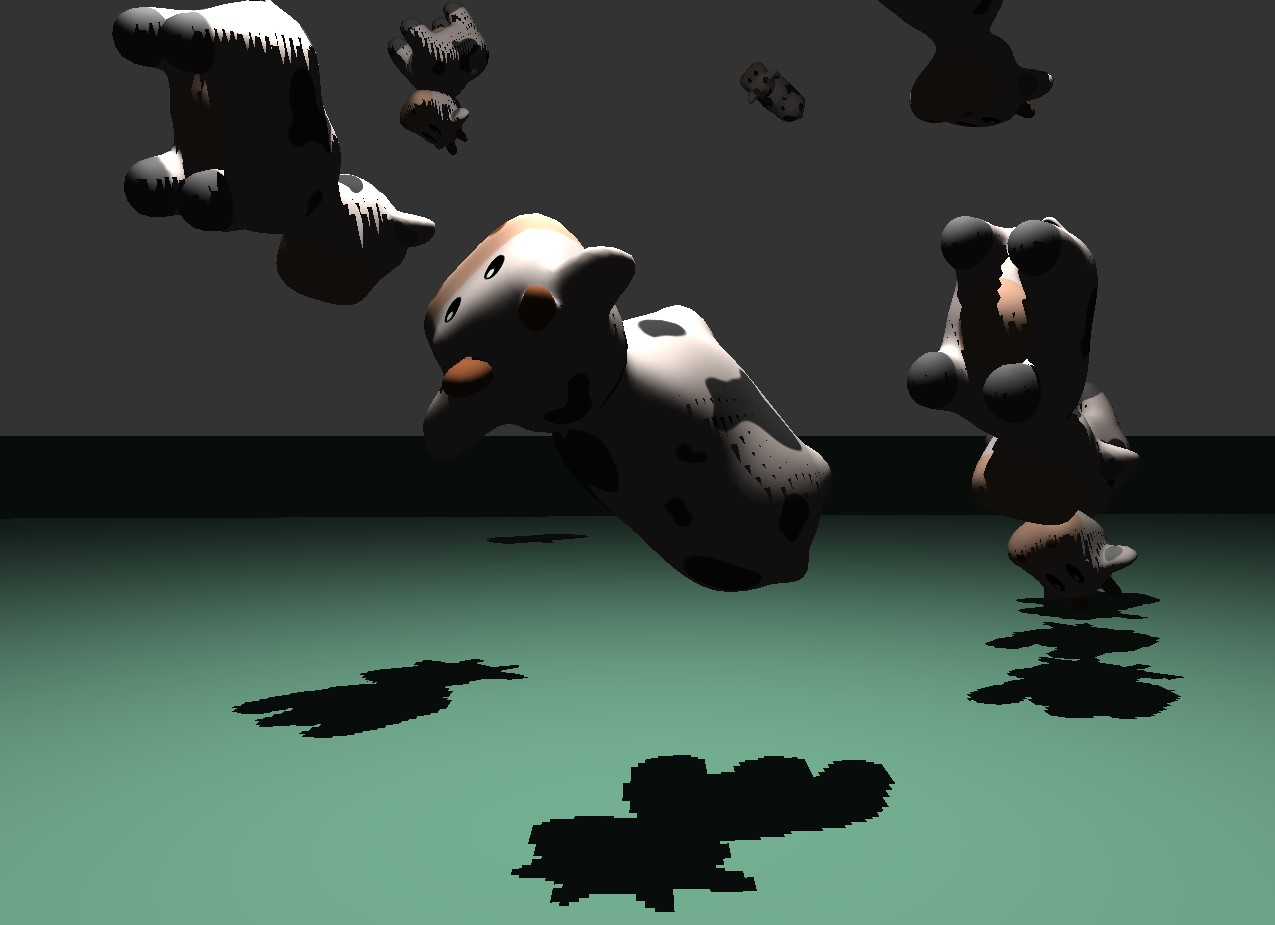
\includegraphics[width=4in]{shadow2.jpg}
			\label{figure.label}
		\end{center}
	\end{figure}

	一个0.005的偏移就能帮到很大的忙,下面的平面已经没有阴影失真了。但是有些表面坡度很大,
	仍然会产生阴影失真。比如奶牛的身上坡度比较大,仍然有阴影失真。
	
	有一个更加可靠的办法能够根据表面朝向光线的角度更改偏移量:使用点乘:
	\begin{framed}
		float bias = max(0.05 * (1.0 - dot(normal, lightDir)), 0.005);
	\end{framed}
	这里我们有一个偏移量的最大值0.05,和一个最小值0.005,它们是基于表面法线和光照方向的
	。下图展示了同一个场景,但使用了点乘的阴影偏移,效果的确更好:
	\begin{figure}[htb]
		\caption{\label{table.label} bias用点乘来计算} \centering
		\begin{center}
			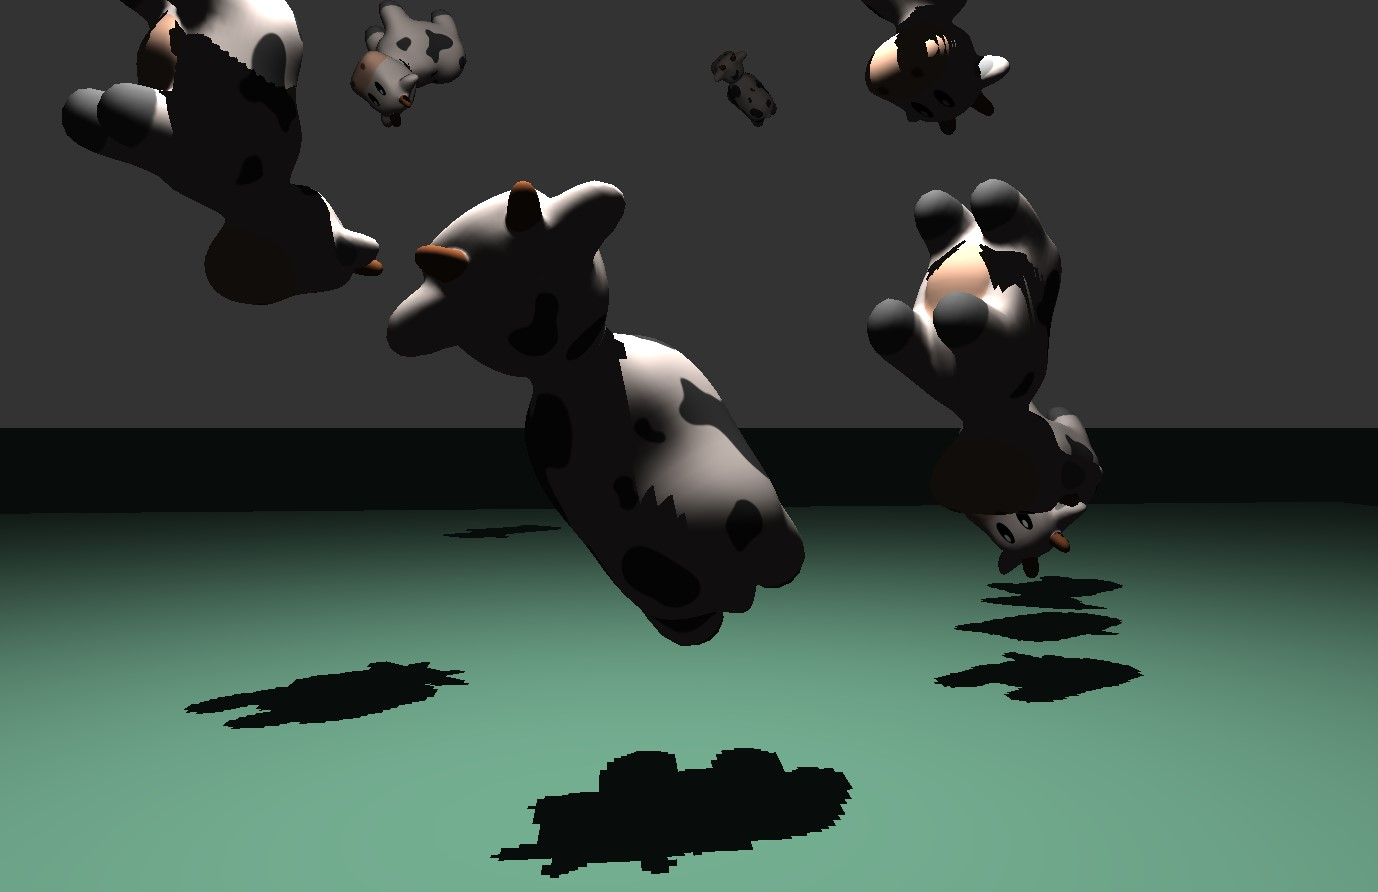
\includegraphics[width=4in]{shadow3.jpg}
			\label{figure.label}
		\end{center}
	\end{figure}

	我们可以看到奶牛身上阴影就没有失真了。
	
	虽然阴影现在已经附着到场景中了,不过这仍不是我们想要的。如果你放大看阴影,阴影映射
	对分辨率的依赖很快变得很明显。因为深度贴图有一个固定的分辨率,多个片段对应于一个纹
	理像素。结果就是多个片段会从深度贴图的同一个深度值进行采样,这几个片段便得到的是同
	一个阴影,这就会产生锯齿边。
	
	我们采用的解决方案叫做PCF(percentage-closer filtering),这是一种多个不同过滤方
	式的组合,它产生柔和阴影,使它们出现更少的锯齿块和硬边。核心思想是从深度贴图中多次
	采样,每一次采样的纹理坐标都稍有不同。每个独立的样本可能在也可能不再阴影中。所有的
	次生结果接着结合在一起,进行平均化,我们就得到了柔和阴影。一个简单的PCF的实现是简单
	的从纹理像素四周对深度贴图采样,然后把结果平均起来:
	\begin{framed}
		float shadow = 0.0;
		
		vec2 texelSize = 1.0 / textureSize(shadowMap, 0);
		
		for(int x = -1; x <= 1; ++x)
		
		\{
			
			for(int y = -1; y <= 1; ++y)
			
			\{
				
				float pcfDepth = texture(shadowMap, projCoords.xy + vec2(x, y) 
				* texelSize).r; 
				
				shadow += currentDepth - bias > pcfDepth ? 1.0 : 0.0; 
				       
			\}    
		
		\}
	
		shadow /= 9.0;
	\end{framed}
	以下为采用PCF后的效果:
	\begin{figure}[htb]
		\caption{\label{table.label} 采用PCF方法} \centering
		\begin{center}
			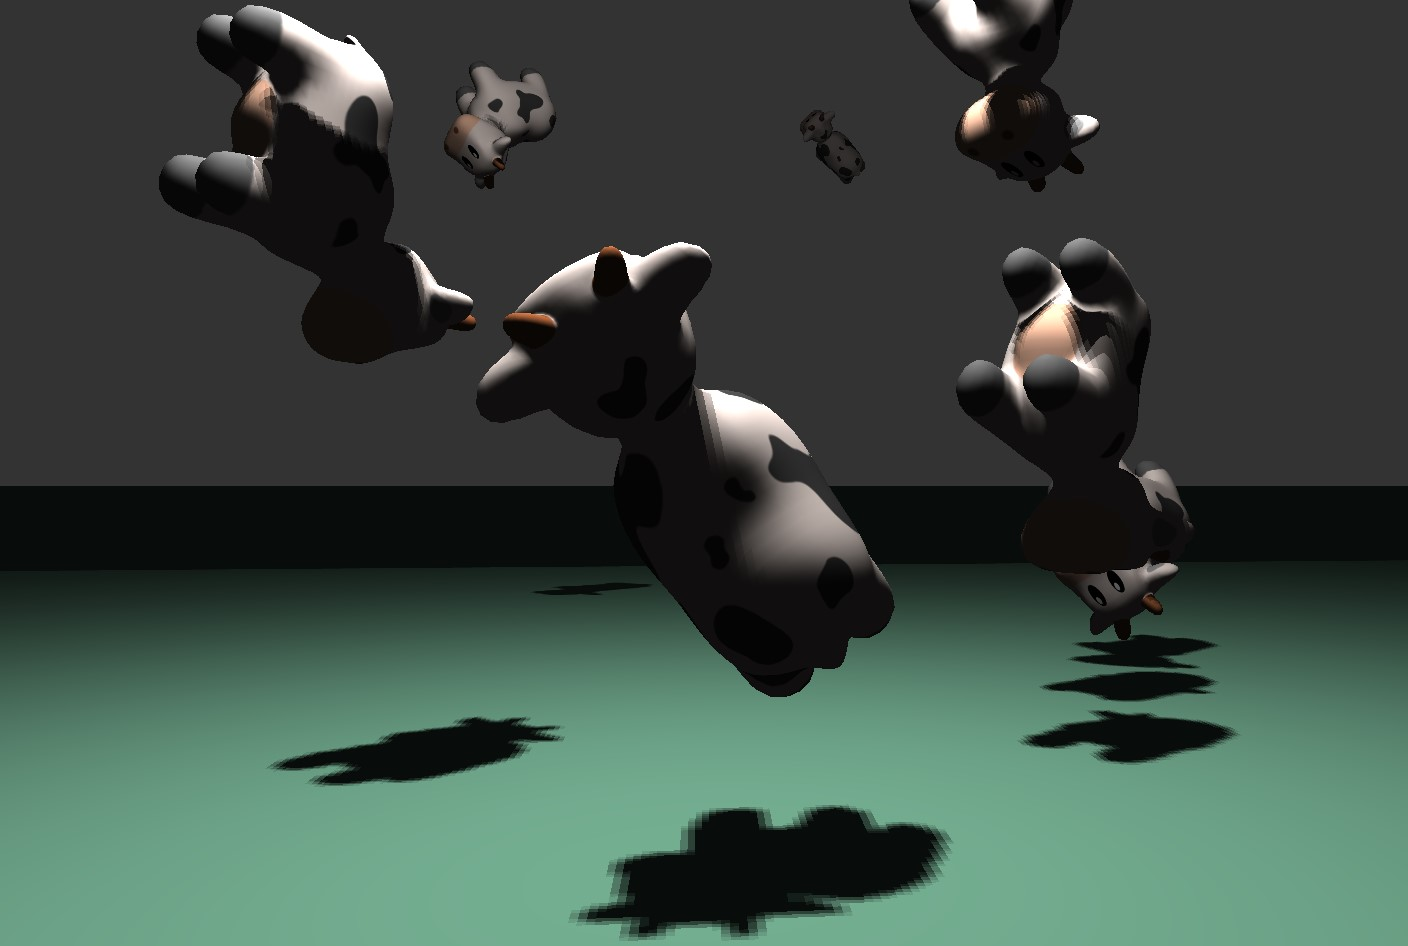
\includegraphics[width=4.7in]{shadow4.jpg}
			\label{figure.label}
		\end{center}
	\end{figure}
	阴影的锯齿边确实好了很多。
	
	以下是在以上优化后的算法基础上,将正交投影改为透视投影的效果:
	\begin{figure}[htb]
		\caption{\label{table.label} 透视投影} \centering
		\begin{center}
			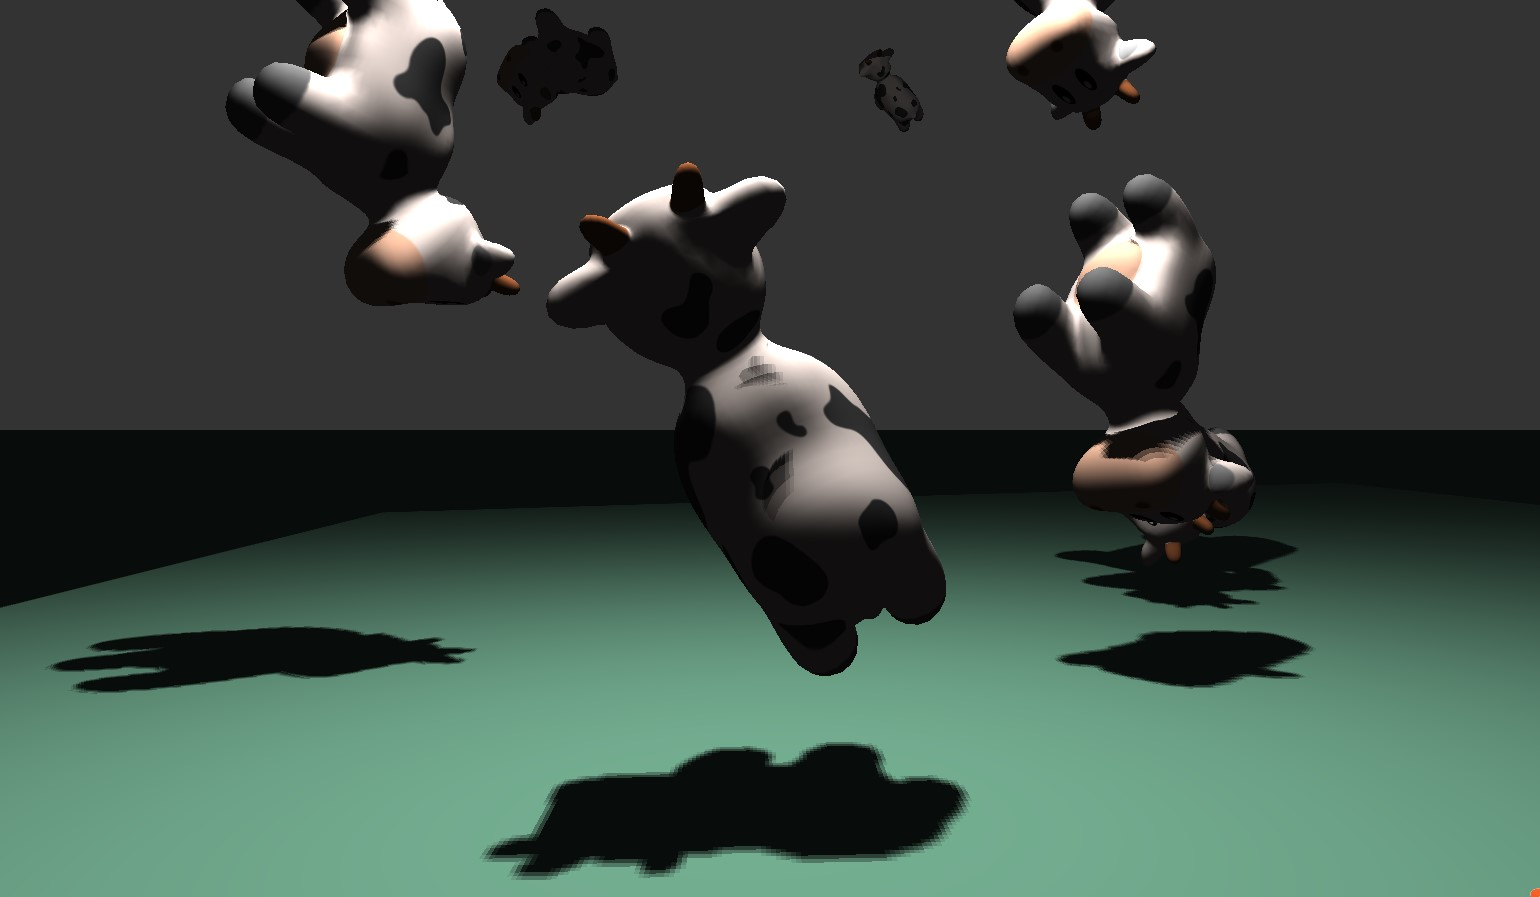
\includegraphics[width=5in]{orth.jpg}
			\label{figure.label}
		\end{center}
	\end{figure}

	\section{不足}
	1. 没有实现更多功能,只实现了最基本的交互和相关功能。
	
	2. 去噪的任务中,不能将裂缝完全消除。

\end{document}
